%\documentclass[prodmode,acmtoms]{acmsmall}
\documentclass[a4paper,10pt]{report}
\usepackage[utf8x]{inputenc}
\usepackage{graphicx}
\usepackage{amsfonts,amsmath,amssymb}


% Title Page
\title{Polynomial class manual}
\author{J. Delgado \and J.M. Pe\~na}


\begin{document}
\maketitle

%\begin{abstract}
%\end{abstract}

\section{Installation}

Extract the contents of the file \verb"Polynomial.zip" into a directory of your choice, e.g. Polynomial-path.
This newly created directory should now be added to the MATLAB path. This can be done temporarly (for 
one MATLAB session) by executing
\begin{verbatim}
 >> addpath (genpath(’Polynomial-path/Polynomial_1.0’))
\end{verbatim}
on the MATLAB command line. The package can also be added to
the MATLAB path permanently via \verb"File/Set Path..." and \verb"Add with Subfolders...". The \verb"Polynomial" package
is now ready for use.

\section{Introduction}

This section describes the structure of the software library. It consists of a Matlab m-file, Polynomial.m, containing the datum definition of the class, 
the declaration of its member functions and operator-overloadings, and of several m-files containing the member functions and the nonmember functions 
used by those. An object of the Polynomial class possesses a piece of private data, \verb"BernsCoeff", the constructor
function \verb"Polynomial", the public member functions \verb"disp", \verb"char", \verb"getDegree", \verb"getCoeff", \verb"double", 
\verb"degreeElevation", \verb"degreeReduction", \verb"Eval", \verb"diff", \verb"integral", \verb"integrate", \verb"plot" and
\verb"subsref", and the overloading
of the operators $+$ (function \verb"plus"), $-$ (function \verb"minus"), $*$ (function \verb"mtimes"), $/$ (function \verb"mrdivide")  
and $\wedge$ (function \verb"mpower").
In addition, the software library also contains the usual functions \verb"Vs", \verb"Casteljau", \verb"CompVs", \verb"Horner",
\verb"TwoSum",  \verb"TwoProduct", \verb"DivRem", \verb"Split", \verb"powerDC", \verb"bd", \verb"interpolation" and \verb"monomial2Bernstein",
implemented each of them in its corresponding m-file, which are used, directly or indirectly, by member functions of the class.
%In the folder \verb"doc" of the software library we have included the file \verb"Manual.pdf" with a description about its use.

In our software library we provide five different ways of constructing a polynomial in Bernstein form.
In contrast to other object oriented languages like C++, Matlab does not allow to overload the constructor
of a class with different input/output arguments. So we have to put the five different ways of constructing a polynomial in Bernstein form
into a unique constructor. We have done it by using the possiblity of accepting any number of input arguments of a function 
in Matlab with \verb"varargin" Matlab variable. The first of the five ways, \verb"Polynomial()", is the default constructor, 
which builds up the zero degree polynomial equal to zero for any 
value of the domain parameter. The copy constructor, invoked by using
\verb"Polynomial(poly)" where \verb"poly" is already an existing object of the polynomial class, returns a copy
of the \verb"poly" object.
In the third way of constructing a polynomial, the user of the library provides a vector $\text{coeff}=(c_0,\ldots,c_n)$ 
with the coefficients of the polynomial respect 
to the Bernstein basis straightforwardly, $p(t)=\sum_{i=0}^n c_ib_i^n(t)$, by using \verb"Polynomial(coeff,'c')", where
\verb"'c'" means control polygon. In Section 3 of the paper we present the mathematical foundations for the two nontrivial ways of constructing polynomials in the Bernstein form, that is, 
from the interpolation conditions (\verb"Polynomial(t,p)") and from the monomial representation (\verb"Polynomial(c,'m')" or \verb"Polynomial(c)").
The design and implementation of the constructor
of the class and the nonmember functions \verb"interpolation", \verb"bd" and \verb"monomial2Bernstein" are presented.
Section 4 of the paper includes a compensated version of the VS algorithm together with a dynamic error estimate. Finally, the design and implementation 
of an adaptative evaluation algorithm \verb"Eval", based in the evaluation algorithms \verb"Vs", \verb"Casteljau" and \verb"CompVs",
is shown in Section 5 of the paper. 

For completeness and usefulness we have included in the software library some other functions. The public member function \verb"getDegree(obj)"
returns the degree of the object \verb"obj" of the Polynomial class. Taking into account that the class data \verb"BernsCoeff" is private, the public 
member functions \verb"getCoeff(obj)" and \verb"double(obj)" return a vector with the coefficients of the object \verb"obj" respect to the Bernstein basis.
We have implemented a private member function \verb"char(obj)", which creates a formatted display of the \verb"Polynomial" object \verb"obj" as
a linear combination of the basis of Bernstein polynomials of the corresponding degree. This formatted display is used by the member 
function \verb"disp(obj)", which determines how Matlab displays a \verb"Polynomial" object \verb"obj" on the command line. 
The member function \verb"subsref(obj)" enables you to specify a value for the independent variable as a subscript, 
access the \verb"BernsCoeff" property with dot notation, and call methods with dot notation. In the public member function
\verb"plot" we overload the usual function in order to plot objects of the \verb"Polynomial" class. A polynomial of a certain
degree $n$ can always be represented exactly as a polynomial of a higher degree. Degree elevation is necessary for the addition 
and substraction of polynomials of different degrees in Bernstein form. The usual method to carry out this degree elevation
for polynomials is shown in \cite{farin} and \cite{BPOLY}, for example. Nevertheless, recently in \cite{S-R} S\'anchez-Reyes has shown the advantages
of performing the degree elevation by using convolution (\verb"conv" function in Matlab). So we have implemented the public member function
\verb"degreeElevation(obj,k)", which performs an elevation of $k$ degrees of the \verb"Polynomial" object \verb"obj" by using \verb"conv".
The differentation and integration of polynomials in Bernstein form are simple operations, which
only involve linear combinations of the Bernstein coefficients of the corresponding polynomial. The formulas for computing
$p'(x)$, $\int p(x)\,dx$ and $\int_0^1 p(x)\,dx$ can be seen in \cite{F-R88}, and the public member functions \verb"diff(obj)",
\verb"integrate(obj)" and \verb"integral(obj)" implement them, respectively. The public member functions \verb"plus(obj1,obj2)" and \verb"minus(obj1,obj2)"
implement the usual addition and subtraction of polynomials, overloading the corresponding operators. First, when necessary, the degree of one of the two polynomials is elevated
by using \verb"degreeElevation(obj,k)" with an adequate $k$. The public member functions \verb"mtimes(obj1,obj2)" and \verb"mpower(obj,k)" implement
the operators $*$ and $\wedge$. In contrast to the usual form, implemented in \cite{BPOLY}, here we also use, like in the case of function \verb"degreeElevation",
Matlab convolution function \verb"conv", which is more efficient as pointed out in \cite{S-R}. 


In the following two sections we show how to use the software package. However, all the following explanations
an commands can be followed in an interactive way through invoking script \verb"manual" (file \verb"manual.m").

\section{Constructing objects of the class}

The \verb"Polynomial" class provides a mold to construct polynomials represented in the basis formed by the Bernstein basis
of degree $n$ given by $b_i^n(x)={n\choose i}x^i(1-x)^{n-i}$. There are five different ways of constructing an object of this class:
\begin{enumerate}
 \item The default constructor, by using \verb"Polynomial()", creates the zero degree polynomial whose value is zero at any point
  \begin{verbatim}
  >> poly1 = Polynomial()
  poly1 = 
  0 
  \end{verbatim}
 \item If $p(x)=\sum_{i=0}^n a_i x^i$ then, by using \verb"Polynomial([a_0,a_1,...,a_n])" or \verb"Polynomial([a_0,a_1,...,a_n],'m')",
  we contruct this polynomial represented in the basis formed by the Bernstein polynomials of degree $n$. So, for the polynomial
  $p(t)=1+2x+3x^2$ it would be
  \begin{verbatim}
  >> poly2 = Polynomial([1,2,3])
  poly2 = 
  bin(2,0)*(1-x)^2 + 2*bin(2,1)*x*(1-x) + 6*bin(2,2)*x^2
  \end{verbatim}
  or
  \begin{verbatim}
  >> poly2 = Polynomial([1,2,3],'m')
  poly2 = 
  bin(2,0)*(1-x)^2 + 2*bin(2,1)*x*(1-x) + 6*bin(2,2)*x^2
  \end{verbatim}  
  \item Given the interpolation conditions $p(x_i)=q_i$, $i=0,1,\ldots,n$, we can construct the interpolating polynomial
  represented in the corresponding Bernstein basis by using \verb"Polynomial([x_0,x_1,...,x_n],[q_0,q_1,...,q_n])". For
  example,
  \begin{verbatim}
>> poly3 = Polynomial([0.25,0.5,0.75],[1,-2,3])
poly3 = 
12*bin(2,0)*(1-x)^2 - 18*bin(2,1)*x*(1-x) + 16*bin(2,2)*x^2
\end{verbatim}   
  creates the polynomial of degree $2$ represented in the Bernstein basis $(b_0^2,b_1^2,b_2^2)$
  satisfying the conditions $p(0.25)=1$, $p(0.5)=-2$ and $p(0.75)=3$.
  \item If the coefficients $c_i$ of the polynomial with respect to the basis formed by the Bernstein polynomial are known
  ($p(t)=\sum_{i=0}^n c_i b_i^n(x)$), the the polynomial can be constructed by using \verb"Polynomial([c_0,c_1,...,c_n],'c')".
  For example,
\begin{verbatim}
>> poly4 = Polynomial(0:1:3,'c')
poly4 = 
bin(3,1)*x(1-x)^2 + 2*bin(3,2)*x^2(1-x) + 3*bin(3,3)*x^3
\end{verbatim}
  \item Finally, the copy constructor:
\begin{verbatim}
>> poly5 = poly2
poly5 = 
bin(2,0)*(1-x)^2 + 2*bin(2,1)*x*(1-x) + 6*bin(2,2)*x^2
\end{verbatim}
  or
\begin{verbatim}
>> poly5 = Polynomial(poly2)
poly5 = 
bin(2,0)*(1-x)^2 + 2*bin(2,1)*x*(1-x) + 6*bin(2,2)*x^2
  \end{verbatim}
\end{enumerate}

\section{Using the methods of the class}

\begin{enumerate}
 \item \verb"getDegree" returns the apparent degree of the polynomial
\begin{verbatim}
>> poly5.getDegree()
ans =
    2
>> poly4.getDegree()
ans =
    3
\end{verbatim}  
  \item \verb"getCoeff" and \verb"double" return the coefficients of the polynomial respect to the Bernstein basis
\begin{verbatim}
>> poly5.getCoeff()
ans =
    1     2     6
>> poly4.double()
ans =
    0     1     2     3
\end{verbatim}  
  \item A polynomial represented in a Bernstein basis can also be represented in a Bernstein basis of greated degree. 
    \verb"degreeElevation" performs this degree elevation. For example the code
\begin{verbatim}
>> poly5 = poly5.degreeElevation(2)

poly5 = 

bin(4,0)*(1-x)^4 + 1.5*bin(4,1)*x(1-x)^3 
 + 2.5*bin(4,2)*x^2(1-x)^2 + 4*bin(4,3)*x^3(1-x) + 6*bin(4,4)*x^4
\end{verbatim}   
  returns the degree 2 polynomial \verb"poly5" represented in the Bernstein basis of degree 4 (=2+2).
  \item Although a polynomial is represented in a Bernstain basis of a certain $n$ degree, the true degree of 
  the polynomial can be lower. The method \verb"degreeReduction" checks the true degree of a polynomial and returns
  the same polynomial represented in the Bernstein basis of the lowest possible degree. For example,
\begin{verbatim}
>> poly5 = poly5.degreeReduction()

poly5 = 

bin(2,0)*(1-x)^2 + 2*bin(2,1)*x*(1-x) + 6*bin(2,2)*x^2
\end{verbatim}  
  \item The usual arithmetic operations can be performed with the usual operators $+$ (sum), $-$ (substraction), $*$ (product),
    $/$ (division) and $\wedge$ (power). Let us see some examples:
\begin{verbatim}
>> poly2+poly4

ans = 

bin(3,0)*(1-x)^3 + 2.6667*bin(3,1)*x(1-x)^2 
 + 5.3333*bin(3,2)*x^2(1-x) + 9*bin(3,3)*x^3
>> poly2-poly4

ans = 

bin(3,0)*(1-x)^3 + 0.66667*bin(3,1)*x(1-x)^2 
 + 1.3333*bin(3,2)*x^2(1-x) + 3*bin(3,3)*x^3
>> poly2*poly4

ans = 

0.6*bin(5,1)*x(1-x)^4 + 1.8*bin(5,2)*x^2(1-x)^3 
 + 4.5*bin(5,3)*x^3(1-x)^2 + 9.6*bin(5,4)*x^4(1-x) 
 + 18*bin(5,5)*x^5
>> [q,r] = poly2/poly4

q = 

0.66667*bin(1,0)*(1-x) + 1.6667*bin(1,1)*x

r = 

1
>> poly6=poly4*q+r

poly6 = 

bin(4,0)*(1-x)^4 + 1.5*bin(4,1)*x(1-x)^3 
 + 2.5*bin(4,2)*x^2(1-x)^2 + 4*bin(4,3)*x^3(1-x) 
 + 6*bin(4,4)*x^4
>> poly6.degreeReduction()

ans = 

bin(2,0)*(1-x)^2 + 2*bin(2,1)*x*(1-x) + 6*bin(2,2)*x^2
>> poly2

poly2 = 

bin(2,0)*(1-x)^2 + 2*bin(2,1)*x*(1-x) + 6*bin(2,2)*x^2
>> poly2^2

ans = 

bin(4,0)*(1-x)^4 + 2*bin(4,1)*x(1-x)^3 
 + 4.6667*bin(4,2)*x^2(1-x)^2 + 12*bin(4,3)*x^3(1-x) 
 + 36*bin(4,4)*x^4
\end{verbatim}  
\item The method \verb"Eval" evaluates a polynomial. It can be invoked in two different ways:
  \verb"Eval(x)" and \verb"Eval(x,prec)". The first one evaluates the polynomial at the points
  in $x$ with a default pretended percision of $10e-12$, whereas the second one performs the
  same evaluation with the pretended precision $prec$. Let us see some examples:
\begin{verbatim}
>> format short e
>> poly4.Eval([0:0.25:1])

ans =

            0   7.5000e-01   1.5000e+00   2.2500e+00   3.0000e+00
          NaN   9.3675e-16   7.7716e-16   6.1062e-16   4.4409e-16
            0   1.0000e+00   1.0000e+00   1.0000e+00   1.0000e+00

>> poly4.Eval([0:0.25:1],5*1e-16)

ans =


            0   7.5000e-01   1.5000e+00   2.2500e+00   3.0000e+00
          NaN   2.2204e-16   2.2204e-16   2.2204e-16   4.4409e-16
            0   1.0000e+00   1.0000e+00   1.0000e+00   1.0000e+00
\end{verbatim}
As we can observe, the method returns for the $1\times 4$ vector of points a $3\times 4$ matrix, where the first row are
consists of the evaluations of the polynomial at the corresponding points in $x$, the second row provides, when possible,
upper bounds of the relative error for the evaluation, and the third row consists of flags (1 means that relative error is lower than $prec$, $0$
means that either relative error is not less than $prec$ or it is not known about). If $x$ is a column vector we obtain 
the traspose matrix: 
\begin{verbatim}
>> poly4.Eval([0;0.25;0.5;0.75;1])

ans =

            0          NaN            0
   7.5000e-01   9.3675e-16   1.0000e+00
   1.5000e+00   7.7716e-16   1.0000e+00
   2.2500e+00   6.1062e-16   1.0000e+00
   3.0000e+00   4.4409e-16   1.0000e+00
\end{verbatim}
The same evaluation can be performed with \verb"obj(x)" or \verb"obj(x,prec)":
\begin{verbatim}
>> poly4(0:0.25:1)

ans =

            0   7.5000e-01   1.5000e+00   2.2500e+00   3.0000e+00
          NaN   9.3675e-16   7.7716e-16   6.1062e-16   4.4409e-16
            0   1.0000e+00   1.0000e+00   1.0000e+00   1.0000e+00

>> poly4(0:0.25:1,5*1e-16)

ans =

            0   7.5000e-01   1.5000e+00   2.2500e+00   3.0000e+00
          NaN   2.2204e-16   2.2204e-16   2.2204e-16   4.4409e-16
            0   1.0000e+00   1.0000e+00   1.0000e+00   1.0000e+00
\end{verbatim}
\item \verb"diff" returns the derivate of a polynomial. For example,
\begin{verbatim}
>> poly7 = poly4.diff()

poly7 = 

3*bin(2,0)*(1-x)^2 + 3*bin(2,1)*x*(1-x) + 3*bin(2,2)*x^2
\end{verbatim}
\item \verb"integrate" returns the indefinite integral of a polynomial.
\begin{verbatim}
>> poly7.integrate()

ans = 

bin(3,1)*x(1-x)^2 + 2*bin(3,2)*x^2(1-x) + 3*bin(3,3)*x^3
\end{verbatim}
\item \verb"integral" returns the definite integral of a polynomial in the interval $[0,1]$:
\begin{verbatim}
>> poly7.integral()

ans =

     3
\end{verbatim}
\item The method \verb"plot" display a graphic of the polynomial in $[0,1]$. This method
  can be invoked in two ways: \verb"plot()" or \verb"plot(step)". The first one, makes
  the graphic taking a mesh of the interval $[0,1]$ with step $0.01$, whereas the second one
  takes a mesh with step \verb"step". Let us see a couple of examples:
\begin{verbatim}
>> poly5.plot()
\end{verbatim}
obtaining the graphic shown in Figure \ref{fig:1}

\begin{figure}[h!]
 \centering
 \includegraphics[scale=0.7]{./figure1.eps}
 % figura1.jpg: 560x420 pixel, 72dpi, 19.76x14.82 cm, bb=0 0 560 420
\caption{Example 1}\label{fig:1}
\end{figure}

and
\begin{verbatim}
>> poly5.plot(0.25)
\end{verbatim}
obtaining the graphic shown in Figure \ref{fig:2}
\begin{figure}[t]
 \centering
 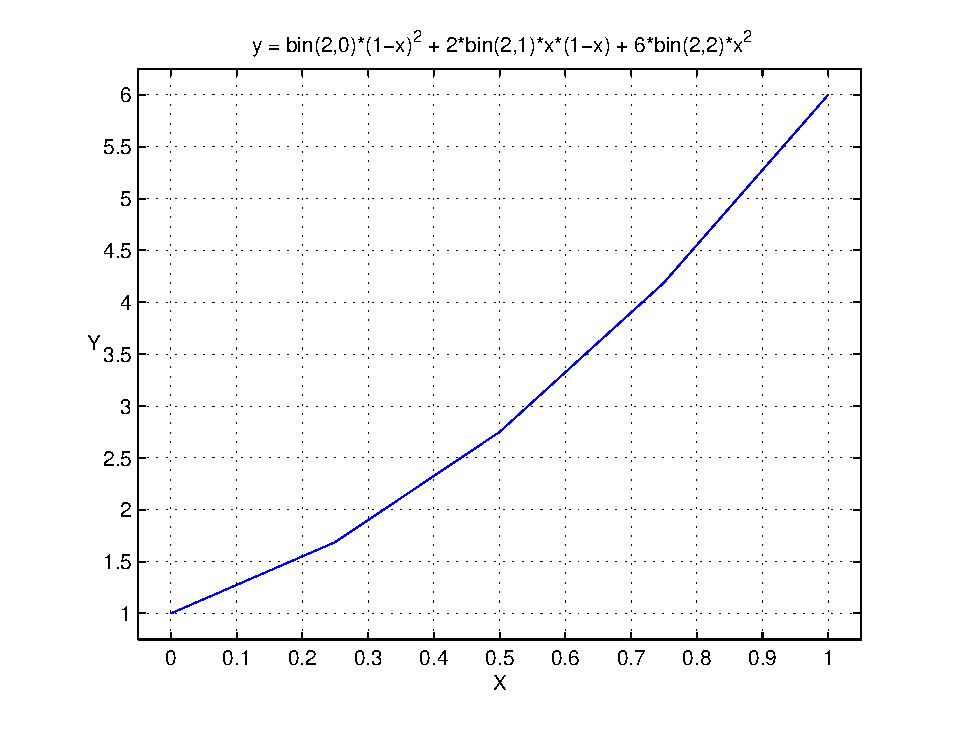
\includegraphics[scale=0.7]{./figure2.eps}
\caption{Example 2}\label{fig:2}
\end{figure}

\end{enumerate}

\section{Test scripts}

In order to test the usefulness of the software package we have included three scripts:
\verb"test1", \verb"test2" and \verb"test3" in the files \verb"test1.m", \verb"test2.m" 
and \verb"test3.m", respectively.

\bibliographystyle{acm}
%\bibliographystyle{ACM-Reference-Format-Journals}
\bibliography{refs.bib}

\end{document}          
